\chapter{Matrix Factorization Methods}  
\label{chap:svd} 


\section{The Goal}

Recall the brief introduction in Chapter \ref{chap:prologue}:  Let $A$
denote the ratings matrix, with the element in row $i$, column $j$
storing the rating of item $j$ given by user $i$.  Say the dimension of
$A$ is $u \times v$ matrix $A$.  We wish to find rank-$k$ matrices $W$
($u \times k$) and $H$ ($k \times v$) such that

\begin{equation}
\label{awh}
A \approx W H
\end{equation}

We typically hope that a good approximation can be achieved with

\begin{equation}
k \ll \textrm{ rank}(A)
\end{equation}

Most importantly, most of the elements of $A$ are unknown.  But because
it is typically the case that similar users have similar ratings
patterns, we hope to obtain good estimates of all of $A$ even though
only a small part of it is known.










The benefits range from compression ($W$ and $H$ are much smaller than
$A$, which in some applications can be huge) to avoidance of
``overfitting'' in a prediction context.

\section{Notation}

We'll use the following notation for a matrix $Q$

\begin{itemize}

\item $Q_{ij}$:  element in row $i$, column $j$

\item $Q_{i \cdot}$:  row $i$

\item $Q_{\cdot j}$:  column $j$

\end{itemize}

Note the key relation

\begin{equation}
(WH)_{.j} = \sum_{i=1}^k H_{ij} W_{.i}
\end{equation}

In other words, in (\ref{awh}), we have that:

\begin{itemize}

\item Column $j$ of $A$ is approximately a linear combination of the
columns of $W$, with the coefficients in that linear combination being
the elements of column $j$ of $H$.  

\item Thus the columns $W_1,...,W_k$ then (approximately) form a basis
for the vector space spanned by the columns of $A$.\footnote{Or, at
least for the nonnegative {\it orthant} in that space, meaning all the
vectors in that space with nonnegative components.}  Since the relation
is only approximate, let's use the term {\it pseudo-basis}.

\item Similarly, we could view everything in terms of rows of $A$ and $H$:
Row $i$ of $WH$ is a linear combination of the rows of $H$, with the
coefficients being row $i$ of $W$.  The rows of $H$ would then be a
pseudo-basis for the rows of $A$.

\item If (\ref{awh}) is a good approximation, then most of the
information carried by $A$ is contained in $W$ and $H$.  We can think of
the columns of $W$ as ``typifying'' those of $A$, with a similar
statement holding for the rows of $H$ and $A$.  Here ``information''
could mean the appearance of an image, the predictive content of data to
be used for machine text classification, and so on.

\end{itemize}

\section{Applications}

This notion of {\it nonnegative matrix factorization} has become widely
used in a variety of applications, such as:

\begin{itemize}

\item Image recognition:

Say we have $n$ image files, each of which has brightness data for
$r$ rows and $c$ columns of pixels.  We also know the class, i.e.\ 
the subject, of each image, say car, building, person and so on.
From this data, we wish to predict the classses of new images. Denote
the class of image $j$ in our original data by $C_j$.

We form a matrix $A$ with $rc$ rows and $n$ columns, where the $i^{th}$
column, $A_{\cdot i}$, stores the data for the $i^{th}$ image, say in
column-major order.  

In the sense stated above, the columns of $W$ typify images.  What about
$H$?  This is a little more complex, though probably more important:

Each image contains information about $rc$ pixels.  The $m^{th}$ of
these, say, varies from image to image, and thus can be thought of as a
random variable in the statistical sense.  Row $m$ in $A$ can be thought
of as a random sample from the population distribution of that random
variable.  

So, the $k$ rows of $H$ typify these $rc$ random variables, and since
$k$ is hopefully much smaller than $rc$, we have received what is called
{\it dimension reduction} among those variables.  It should be
intuitively clear that this is possible, because there should be a high
correlation between neighboring pixels, thus a lot of ``redundant''
information.

This is very important with respect to the {\it overfitting} problem in
statistics/machine learning.  This is beyond the scope of this tutorial,
but the essence of fhe concept is that having too complex a model can
lead to ``noise fitting,'' and actually harm our goal of predicting the
class of future images.  By having only $k$ rows in $H$, we are reducing
the dimensionality of the problem from $rc$ to $k$, thus reducing the
chance of overfitting.

Our prediction of new images works as follows.  Given the $rc$-element
vector $q$ of the new image of unknown class, we find its representation
$q_p$ in the pseudo-basis for the rows of $A$, and then find
$g$ such $G_{g \cdot}$ best matches $q_p$.  Our predicted class is then
$C_g$.

\item Text classification:

Here $A$ consists of, say, word counts. We have a list of $d$ key words,
and $m$ documents of known classes (politics, finance, sports etc.).
$A_{ij}$ is the count of the number of times word $i$ appears in
document $j$.

Otherwise, the situation is the same as for image recognition above.  We
find the NMF, and then given a new document to classify, with word
counts $q$, we find its coordinates $q_p$, and then predict class by
matching to the rows of $W$.

\item Recommender systems:

Here most of $A$ is unknown.  For instance, we have users, who have
rated movies they've seen, with $A_{ij}$ being the rating of movie $j$
by user $i$.  Our goal is to fill in estimates of the unknown entries.

One approach is to initially insert 0s for those entries, then perform
NMF, producing $W$ and $H$.\footnote{A popular alternative uses {\it
stochastic gradient} methods to find the best fit directly, without
creating the matrix $A$.} We then compute $WH$ as our estimate of $A$,
and now have estimates for the missing entries.

\end{itemize}

\section{The R Package NMF}

The R package {\bf NMF} is quite extensive, with many, many options.  In
its simplest form, though, it is quite easy to use.  For a matrix {\bf
a} and desired rank {\bf k}, we simply run

\begin{lstlisting}
> nout <- nmf(a,k)
\end{lstlisting}

Here the returned value {\bf nout} is an object of class {\bf "NMF"}
defined in the package.  It uses R's S4 class structure, with
\lstinline{@} as the delimiter denoting class members.  

As is the case in many R packages, {\bf "NMF"} objects contain classes
within classes.  The computed factors are in {\bf nout@fit@W} and {\bf
nout@fit@H}.

Let's illustrate it in an image context, using the following:

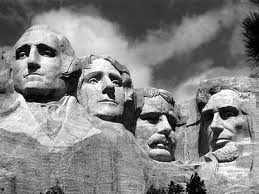
\includegraphics[width=3.6in]{Images/MtRush.png}

Here we have only one image, and we'll use NMF to compress it, not do
classification.  First obtain $A$:

\begin{lstlisting}
> library(pixmap) 
# read file
> mtr <- read.pnm('MtRush.pgm') 
> class(mtr)
[1] "pixmapGrey"
attr(,"package")
[1] "pixmap"
# mtr is an R S4 object of class "pixmapGrey"
# extract the pixels matrix
> a <- mtr@grey
\end{lstlisting}

Now, perform NMF, find the approximation to $A$, and display it:

\begin{lstlisting}
> aout <- nmf(a,50)
> w <- aout@fit@W
> h <- aout@fit@H
> approxa <- w %*% h
# brightness values must be in [0,1]
> approxa <- pmin(approxa,1) 
> mtrnew <- mtr
> mtrnew@grey <- approxa 
> plot(mtrnew) 
\end{lstlisting}

Here is the result:

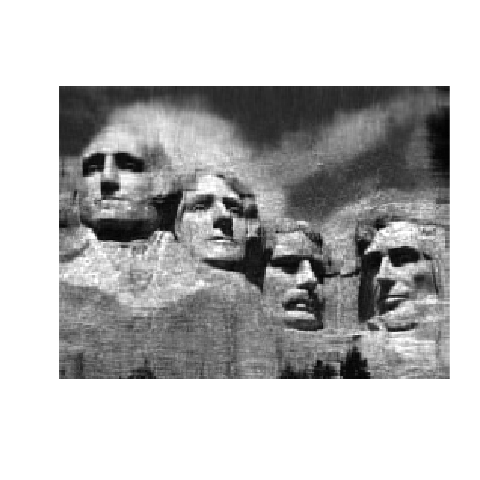
\includegraphics[width=3.6in]{Images/MtRush50.png}

This is somewhat blurry.  The original matrix has dimension $194
\times 259$, and thus presumably has rank 194.\footnote{This is
confirmed by running the function {\bf rankMatrix()} in the {\bf Matrix}
package.} We've approximated the matrix by one of rank only 50, a
storage savings.  Not important for one small picture, but possibly
worthwhile if we have many. The approximation is not bad in that light,
and may be good enough for image recognition or other applications.

\section{Algorithms}

How are the NMF solutions found?  What is {\bf nmf()} doing internally?

Needless to say, the methods are all iterative, with one approach being
that of the Alternating Least Squares algorithm.  By the way, this is
not the default for {\bf nmf()}; to select it, set {\bf method =
'snmf/r'}.

\subsection{Objective Function}

We need an {\it objective function}, a criterion to optimize, in this
case a criterion for goodness of approximation. Here we will take that
to be the {\it Frobenius} norm, which is just the Euclidean ($L_2$)
norm with the matrix treated as a vector:\footnote{The $L_p$ norm of a
vector $v = (v_1,...,v_r)$ is defined to be

$$
\left (\sum_i |v_i|^p \right )^{1/p}
$$
}

\begin{equation}
\|Q\|_2 = 
\sqrt{
\sum_{i,j} Q_{ij}^2
}
\end{equation}

So our criterion for error of approximation will be

\begin{equation}
\label{errawh}
\|A - WH\|_2
\end{equation}

This measure is specified in {\bf nmf()} by setting {\bf objective =
'euclidean'}.

\subsection{Alternating Least Squares}

So, how does it work?  It's actually quite simple.  Suppose just for a
moment that we know the exact value of $W$, with $H$ unknown.  Then for
each $j$ we could minimize

\begin{equation}
\label{errajwhj}
\|A_{\cdot j} - W H_{\cdot j}\|_2
\end{equation}

We are seeking to find $H_{\cdot j}$ that minimizes (\ref{errajwhj}),
with $A_{\cdot j}$ and $W$ known.  But since the Frobenius norm is just
a sum of squares, that minimization is just a least-squares problem,
i.e.\ {\it linear regression}; we are ``predicting'' $A_{\cdot j}$ from
$W$.  The solution is well-known to be\footnote{If you have background
in regression analysis, you might notice there is no constant term,
$\beta_0$, here.}

\begin{equation}
H_{\cdot j} = (W'W)^{-1} W' A_{\cdot j}
\end{equation}

R's {\bf lm()} function does this for us

\begin{lstlisting}
> h[,j] <- lm(a[,j] ~ w - 1)
\end{lstlisting}

for each $j$.\footnote{The -1 specifies that we do not want a constant term in
the model.}

On the other hand, suppose we know $H$ but not $W$.  We could take 
transposes,

\begin{equation}
A' = H' W'
\end{equation}

and then just interchange the roles of $W$ and $H$ above.  Here a call
to {\bf lm()} gives us a row of $W$, and we do this for all rows.

Putting all this together, we first choose initial guesses, say random
numbers, for $W$ and $H$; {\bf nmf()} gives us various choices as to how
to do this.  Then we alternate: Compute the new guess for $W$ assuming
$H$ is correct, then choose the new guess for $H$ based on that new $W$,
and so on.

During the above process, we may generate some negative values.  If so,
we simply truncate to 0.

\subsection{Multiplicative Update}

Alternating Least Squares is appealing in several senses.  At each
iteration, it is minimizing a {\it convex} function, meaning in essence
that there is a unique local and global minimum; it is easy to
implement, since there are many least-squares routines publicly
available, such as {\bf lm()} here; and above all, it has a nice
interpretation, predicting columns of $A$.

Another popular algorithm is {\it multiplicative update}, due to Lee and
Seung.  Here are the update formulas for $W$ given $H$ and {\it vice
versa}:

\begin{equation}
W \leftarrow W \circ 
\frac
{AH'}
{WHH'}
\end{equation}

\begin{equation}
H \leftarrow H \circ 
\frac
{W'A}
{W'WH}
\end{equation}

where $Q \circ R$ and $\frac{Q}{R}$ represent \underline{elementwise}
multiplication and division with conformable matrices $Q$ and $R$, and
the juxtaposition $QR$ means ordinary matrix multiplication.

\section{Predicting New Cases}

Once we have settled on $W$ and $H$, what can we do with them?  In the
recommender system application mentioned earlier, we simply multiply
them, and then retrieve the predicted values at the matrix positions at
which we did not have user ratings.  But recall the description given
above for the image and text processing examples: 

\begin{quote}
Given the $rc$-element vector $q$ of the new image, we find
its representation $q_p$ in the pseudo-basis, and then find $g$ such
$W_{g \cdot}$ best matches $q_p$.  Our predicted class is then $C_g$.
\end{quote}

How do we find $q_p$?  The answer is that again we can use the
least-squares above.

\begin{lstlisting}
> qp <- lm(q ~ h - 1)
\end{lstlisting}

\section{Convergence and Uniqueness Issues}

There are no panaceas for applications considered here.  Every solution
has potential problems.

With NMF, an issue may be uniqueness --- there might not be a unique
pair $(W,H)$ that minimizes (\ref{errawh}).\footnote{See Donoho and
Stodden,{\it When Does Non-Negative Matrix Factorization Give a Correct
Decomposition into Parts?},
\url{https://web.stanford.edu/~vcs/papers/NMFCDP.pdf}.  } In turn, this
may result in convergence problems. The NMF documentation recommends
running {\bf nmf()} multiple times; it will use a different seed for the
random initial values each time.

The Alternating Least Squares method used here is considered by some to
have better convergence properties, since the solution at each iteration
is unique.  

\section{How Do We Choose the Rank?}

This is not an easy question.  One approach is to first decompose our
matrix $A$ via {\it singular value decomposition}.  Roughly speaking,
SVD finds an orthonormal basis for A, but then treats the vectors in
that basis as random variables.  The ones with relatively small variance
may be considered unimportant.

\begin{lstlisting}
> asvd <- svd(a)
> asvd$d
  [1] 1.188935e+02 2.337674e+01 1.685734e+01 1.353372e+01 1.292724e+01
  [6] 1.039371e+01 9.517687e+00 9.154770e+00 8.551464e+00 7.776239e+00
 [11] 6.984436e+00 6.505657e+00 5.987315e+00 5.059873e+00 5.032140e+00
 [16] 4.826665e+00 4.576616e+00 4.558703e+00 4.107498e+00 3.983899e+00
 [21] 3.923439e+00 3.606591e+00 3.415380e+00 3.279176e+00 3.093363e+00
 [26] 3.019918e+00 2.892923e+00 2.814265e+00 2.721734e+00 2.593321e+00
\end{lstlisting}

So, the first standard deviation is about 119, the next about 23 and so
on.  The seventh is already down into the single-digit range.  So we
might take $k$ to be, say, 10.  The columns of $A$ lie in a subspace of
$R^{194}$ of dimension of about 10.

\section{Why Nonnegative?}

In the applications we've mentioned here, we always have $A \geq 0$.
However, that doesn't necesarily mean that we need $W$ and $H$ to be
nonnegative, since we could always truncate.  Indeed, we could consider
using SVD instead.

There are a couple of reasons NMF may be preferable.  First, truncation
may be difficult if we have a lot of negative values.  But the second
reason is rather philosophical, as follows:

In the image recognition case, there is hope that the vectors $W_{\cdot
j}$ will be {\it sparse}, i.e.\ mostly 0s. Then we might have, say, the
nonzero elements of $W_{\cdot 1}$ correspond to eyes, $W_{\cdot 2}$
correspond to nose and so on with other parts of the face.  We are then
``summing'' to form a complete face.  This may enable effective {\it
parts-based recognition}.

Sparsity (and uniqueness) might be achieved by using {\it
regularization} methods, in which we minimize something like

\begin{equation}
\|A - WH\| + \lambda (\|W\|_1 + \|H\|_1)
\end{equation}

where the subscript 1 (``$L_1$ norm'') means the norm involves sums of
absolute values rather than sums of squares.  This guards against one of
the factors becoming ``too large,'' and it turns out that this also can
lead to sparse solutions.  We can try this under {\bf nmf()}  by setting
{\bf method = 'pe-nmf'}.


